
\chapter{PRE-PROCESSING} 
Various preprocessing techniques were applied to the given data set, and all the proposed models were built on this data. The PIMA Indian Diabetes dataset was found to have 0 values for certain attributes, which doesn't comply with common sense in real life. Thus, these ``0 values" were treated as missing data, and were handled using different methodologies. Specifically, with respect to our dataset, the following were the attributes with the above mentioned characteristics:
\begin{itemize}
    \item Glucose
    \item Blood Pressure
    \item Skin Thickness
    \item Insulin
    \item BMI
\end{itemize}

The pre-processing techniques employed on the data can be broadly classified into two categories:
\begin{itemize}
    \item Handling the missing values ( “0 values” in the above specified attribute list)
    \item Normalizing the data

\end{itemize}

\section{Methodologies Employed}
Techniques for handling missing data  include:
\begin{itemize}
    \item \textbf{Filling the zero values with mean:}
The attributes with missing values were first replaced with ``nan" ( not a number ), and ``nan" was subsequently replaced with the mean of each corresponding attribute.
    \item\textbf{Filling the zero values with median:}
The attributes with missing values were first replaced with ``nan" ( not a number ), and ``nan" was subsequently replaced with the median of each corresponding attribute.

\item \textbf{Dropping the rows containing attributes with these missing values:}
The attributes with missing values were first replaced with ``nan" ( not a number ), and rows with ``nan" were subsequently dropped. The size of the dataset reduced to almost 50\% of the initial size.

\item \textbf{Using the k-nearest neighbour classifier to fill appropriate values:}
A KNN model was built for each and every attribute with missing values separately. These models were used to predict the probable values for the corresponding attribute's missing data.
\end{itemize}

Normalization of data was done using PCA (Principal Component Analysis), and the number of resultant components was fixed as 8, which is the same as the number of input attributes. The various preprocessing techniques against the different models along with evaluation parameters have been tabulated in Table 3.1.


\begin{adjustbox}{angle=90}
\scalebox{0.87}{
    \begin{tabular}{|c|c|c|c|c|c|c|}
    \hline
    \textbf{MODEL} & \textbf{PRE PROCESSING} & \textbf{ACCURACY} & \textbf{SENSITIVITY} & \textbf{SPECIFICITY} & \textbf{PRECISION} &	\textbf{ERROR RATE} \\ 
    \hline     
    \multirow{ID3} & Mean & 79.87 & 70.21 & 84.11 & 66 & 20.13\\
    & Median & 74.68 & 72.34 & 75.7 & 56.67 & 25.32\\
    & Dropping & 75.95 & 52 & 87.03 & 65 & 24.05\\
    & KNN & 80.51 &	61.7 & 88.78 & 70.73 & 19.49\\
    & KNN + PCA & 68.18 & 59.57 & 70.96 & 48.27 & 31.82\\
    \hline
    \multirow{CART} & Mean & 78.57 & 65.95 & 84.11 & 64.58 & 21.43\\
    & Median & 78.57 &	65.95 &	84.11 &	64.58 &	21.43\\
    & Dropping	& 78.48 & 60 & 87.03 &	68.18 &	21.52\\
    & KNN &	72.07 &	57.44 & 78.5 &	54 &	27.93\\
    & KNN + PCA	& 68.83 & 61.7 & 71.96 & 49.15 & 31.17\\
    \hline
    \multirow{C4.5} & Mean & 77.27 & 62.96 & 85 & 69.39 & 22.73\\
    & Median & 77.27 & 62.96 & 85 &	69.39 &	22.73\\
    & Dropping & 66.67 & 46.15 & 76.92 & 50 & 33.33\\
    & KNN &	77.27 &	62.96 &	85 & 69.39 & 22.73\\
    \hline
    \multirow{ANN} & Mean & 81.17 &	76.59 &	83.17 &	66.66 &	18.83\\
    & Median &	80.52 &	59.57 &	89.72 & 71.79 &	19.48\\
    & Dropping & 81.01 & 68	& 87.04 & 70.83 & 18.99\\
    & KNN &	74.03 &	65.96 &	77.57 & 56.36 &	25.97\\
    & KNN + PCA	& 81.82 & 48.94 & 96.26 & 85.18 & 18.18\\
    \hline
    \end{tabular}}
    
\end{adjustbox}
\captionof{table}{All preprocessing techniques, models and evaluation metrics}
%\newpage
\clearpage
\begin{figure}[h]
%\vspace{-3.8in}
\centering %\offinterlineskip
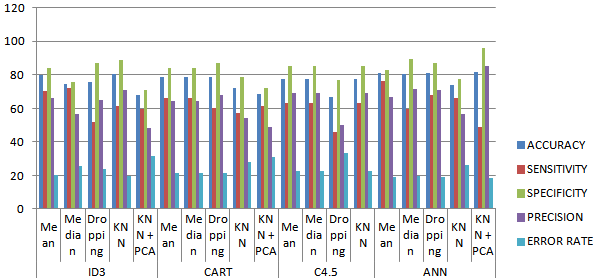
\includegraphics[scale=1.15]{sumprp4.PNG}
\caption{\label{fig:subBDDs1}Summary of all pre-processing techniques, models and parameters}
\end{figure}
\par \noindent The Table 3.1 has been briefly summarized in Figure 3.1.
%\pagebreak
Figure 3.2 summarizes the results obtained from the top two pre-processing techniques for each model.
\begin{figure}[h]
%\vspace{-3.8in}
\centering %\offinterlineskip
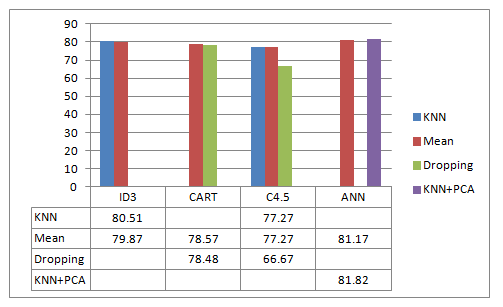
\includegraphics[scale=1.15]{topprp.PNG}
\caption{\label{fig:subBDDs1}Top two pre-processing technique for all models
based on accuracy
}
\end{figure}
\pagebreak
\section{Consensus}
In the above tabulation, the best pre-processing technique (decided based on the model accuracy) for a model, it can be observed that \textbf{mean} is the only preprocessing technique that occurs as either the best or the second-to-best preprocessing method for all the models. Hence filling the missing values with mean was the only data preprocessing technique, that was applied to our dataset.